% !TEX root = ../memoire.tex
\chapter{Fondements Théoriques : Le Modèle LWR de Base}
\label{chap:fondements_theoriques}

\section{Principes du Modèle LWR}
\label{sec:principes_lwr}

Le modèle macroscopique de trafic routier développé indépendamment par Lighthill et Whitham \cite{lighthill1955kinematic} et Richards \cite{richards1956shock}, communément appelé modèle LWR, constitue l'un des fondements de la théorie moderne de l'écoulement du trafic. Ce modèle s'appuie sur trois principes fondamentaux :

\begin{itemize}
    \item Le \textbf{principe de conservation de la masse}  : Ce principe stipule que le nombre de véhicules est conservé, c'est-à-dire qu'il n'y a ni création ni disparition de véhicules sur le tronçon de route considéré. Mathématiquement, cela se traduit par une équation de continuité reliant la densité du trafic et le flux de véhicules.
    \item L'\textbf{hypothèse d'une relation fonctionnelle entre le flux et la concentration}  : Le modèle LWR repose sur l'hypothèse fondamentale qu'il existe une relation unique et déterministe entre le flux de trafic (le nombre de véhicules passant un point donné par unité de temps) et la concentration (la densité de véhicules sur la route). Cette relation est généralement représentée par un diagramme fondamental, qui peut varier en fonction des conditions de la route [4].
    \item Le \textbf{principe de l'écoulement continu} : Ce principe considère le trafic comme un fluide continu, ce qui permet d'appliquer les équations de la dynamique des fluides pour décrire son comportement macroscopique. Cette approche est valide lorsque le nombre de véhicules est suffisamment élevé pour que les fluctuations individuelles soient négligeables.
\end{itemize}

\begin{definition}[Approche continue du trafic]
    L'approche macroscopique considère le trafic comme un flux continu caractérisé par des variables agrégées (densité, vitesse moyenne, flux) plutôt que par les trajectoires individuelles des véhicules.
    \end{definition}
    
    Le modèle LWR repose sur plusieurs hypothèses simplificatrices :
    
    \begin{itemize}
        \item \textbf{Le trafic est homogène} : Cette hypothèse suppose que les caractéristiques de la route (nombre de voies, largeur, etc.) et le comportement des conducteurs sont uniformes sur le tronçon considéré [1].
        \item \textbf{Il existe une relation unique entre la densité et le flux} : Le modèle LWR postule une relation déterministe et statique entre la densité du trafic et le flux, généralement représentée par le diagramme fondamental [2, 3].
        \item \textbf{Les effets d'inertie et de relaxation sont négligeables} : Le modèle suppose que les conducteurs réagissent instantanément aux changements de densité, sans délai ni inertie [4].
        \item \textbf{Il n'y a ni entrées ni sorties intermédiaires} : Le modèle de base considère un tronçon de route sans jonctions, entrées ou sorties intermédiaires, où les véhicules entrent à une extrémité et sortent à l'autre [1].
        \item \textbf{La vitesse est une fonction de la seule densité} : le modèle suppose que la vitesse des véhicules ne dépend que de la densité locale et non d'autres facteurs tels que l'historique du trafic ou les conditions en aval [5].
    \end{itemize}

Ces hypothèses, bien que restrictives, permettent d'obtenir un modèle mathématiquement tractable qui capture les phénomènes essentiels du trafic, notamment la formation et la propagation des congestions.

\section{Variables et Équation de Conservation}
\label{sec:equation_conservation}

Le modèle LWR s'articule autour de trois variables macroscopiques fondamentales, définies comme des fonctions continues de la position $x$ et du temps $t$ :

\begin{definition}[Variables macroscopiques]
\begin{itemize}
\item La \textbf{densité} $\dens(x,t)$ : nombre de véhicules par unité de longueur (véh/km);
\item La \textbf{vitesse moyenne} $\vel(x,t)$ : vitesse moyenne des véhicules à la position $x$ au temps $t$ (km/h);
\item Le \textbf{flux} $\flow(x,t) = \dens(x,t) \cdot \vel(x,t)$ : nombre de véhicules traversant un point par unité de temps (véh/h).
\end{itemize}
\end{definition}

L'équation fondamentale du modèle LWR est l'équation de conservation, issue du principe de conservation des véhicules :

\begin{empheq}[box=\colorbox{lightblue!15}]{align}
\pd{\dens}{t} + \pd{(\dens \vel)}{x} = 0 \quad \text{ou} \quad \pd{\dens}{t} + \pd{\flow}{x} = 0.
\label{eq:conservation_lwr}
\end{empheq}

Cette équation stipule que la variation temporelle de la densité (terme $\pd{\dens}{t}$) additionnée à la variation spatiale du flux (terme $\pd{\flow}{x}$ ou $\pd{(\dens \vel)}{x}$) doit être nulle en l'absence de sources ou de puits. **Elle exprime la conservation du nombre de véhicules : tout changement de densité en un point est dû à une différence de flux entre ce qui entre et ce qui sort de ce point.**

\begin{remark}
L'équation de conservation est une équation aux dérivées partielles (EDP) du premier ordre, de type hyperbolique. Cette nature hyperbolique est responsable de la formation d'ondes de choc dans le trafic, correspondant aux fronts de congestion. **Ces ondes de choc se produisent lorsque le trafic de faible densité rattrape un trafic plus dense et plus lent en aval** [1, 2].
\end{remark}

\section{Diagramme Fondamental et Relation Vitesse-Densité}
\label{sec:diagramme_fondamental}

Pour résoudre l'équation de conservation du modèle LWR, il est nécessaire de spécifier la relation entre le flux $\flow$ (ou la vitesse $\vel$) et la densité $\dens$, connue sous le nom de \textit{relation fondamentale du trafic} ou \textit{diagramme fondamental}.

Le diagramme fondamental établit la relation entre la densité et le flux (ou la vitesse) du trafic. Cette relation est essentielle pour fermer le système d'équations et rendre l'équation de conservation soluble. **Il représente une simplification de la réalité, car il suppose une relation statique et déterministe entre ces variables macroscopiques** [1].

\begin{figure}[htbp]
\centering
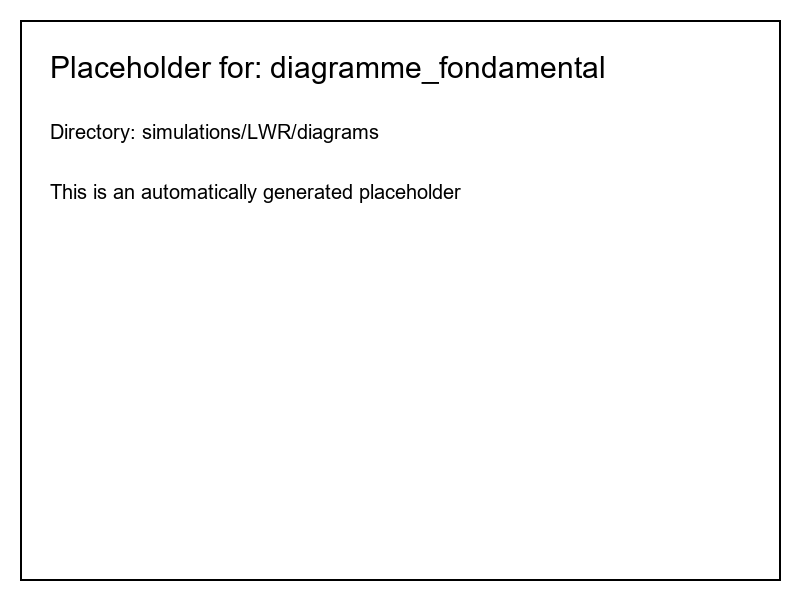
\includegraphics[width=1.0\textwidth]{simulations/LWR/diagrams/diagramme_fondamental}
\caption{Diagrammes fondamentaux du modèle LWR selon Greenshields : (a) relation vitesse-densité montrant la décroissance linéaire de la vitesse avec la densité, (b) relation flux-densité montrant la forme parabolique caractéristique avec le point critique à $\rho_c = \rho_{\max}/2$, et (c) relation flux-vitesse.}
\label{fig:diagramme_fondamental}
\end{figure}

\subsection{Le Modèle de Greenshields}
\label{subsec:greenshields}

La relation la plus simple et la plus utilisée est celle proposée par Greenshields \cite{greenshields1935study}, qui postule une relation linéaire entre la vitesse et la densité :

\begin{empheq}[box=\colorbox{lightblue!15}]{align}
\vel(\dens) = \maxvel \left(1 - \frac{\dens}{\maxdens}\right)
\label{eq:greenshields_vitesse}
\end{empheq}

où $\maxvel$ représente la vitesse maximale (ou vitesse en flux libre) et $\maxdens$ la densité maximale (ou densité de blocage).

En utilisant le modèle de Greenshields, la relation entre le flux et la densité se dérive de la combinaison de la relation linéaire vitesse-densité avec la définition du flux:
$$\flow(\dens) = \dens \cdot \vel(\dens)$$

En substituant l'équation de vitesse de Greenshields, on obtient :
\begin{align}
\flow(\dens) &= \dens \cdot \maxvel \left(1 - \frac{\dens}{\maxdens}\right) \notag \\
&= \maxvel \dens - \frac{\maxvel}{\maxdens} \dens^2
\label{eq:greenshields_flux}
\end{align}

Cette équation révèle une relation parabolique entre le flux et la densité. Le flux est nul lorsque la densité est nulle (route vide) ou égale à la densité maximale $\maxdens$ (congestion maximale, embouteillage). Le flux maximal, correspondant à la capacité de la route, est atteint lorsque la densité est égale à la moitié de la densité maximale.

\begin{figure}[htbp]
\centering
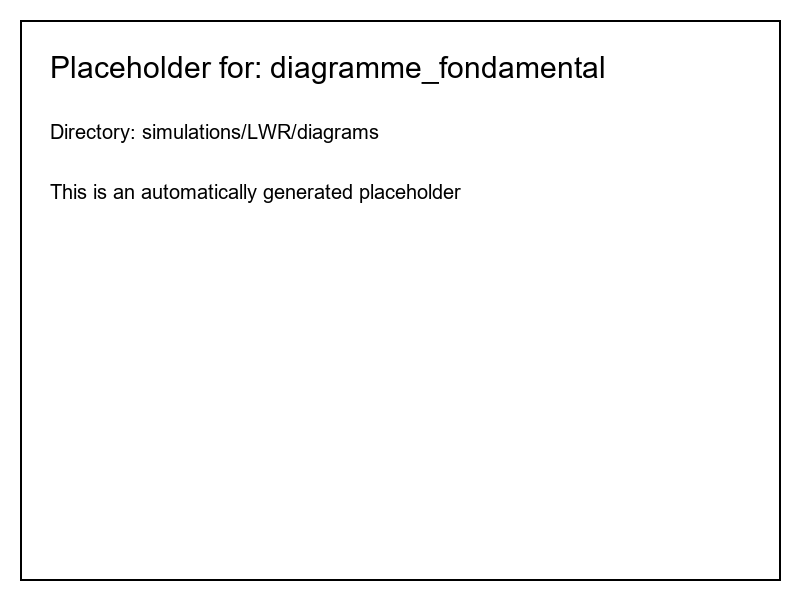
\includegraphics[width=1.0\textwidth]{simulations/LWR/diagrams/diagramme_fondamental}
\caption{Diagrammes fondamentaux du modèle LWR selon Greenshields : (a) relation vitesse-densité montrant la décroissance linéaire de la vitesse avec la densité, (b) relation flux-densité montrant la forme parabolique caractéristique avec le point critique à $\rho_c = \rho_{\max}/2$, et (c) relation flux-vitesse.}
\label{fig:diagramme_fondamental}
\end{figure}

\subsection{Régimes de Circulation}
\label{subsec:regimes}

Le diagramme fondamental permet d'identifier trois régimes de circulation principaux :

\begin{enumerate}
    \item \textbf{Régime fluide (ou non congestionné)} : caractérisé par une faible densité, une vitesse élevée, et une augmentation du flux avec la densité. Dans ce régime, les véhicules peuvent circuler librement, et l'augmentation du nombre de véhicules sur la route entraîne une augmentation du flux total.
    \item \textbf{Régime critique} : correspond à une densité intermédiaire, où le flux atteint son maximum (capacité de la route). Ce point représente l'utilisation optimale de la route, où le nombre de véhicules est maximisé sans pour autant entraîner de congestion.
    \item \textbf{Régime congestionné} : caractérisé par une forte densité, une vitesse réduite, et une diminution du flux avec l'augmentation de la densité. Dans ce régime, l'ajout de véhicules supplémentaires ne fait qu'aggraver la congestion et réduire le flux total. Les **ondes cinématiques** et les **ondes de choc cinématiques** sont courantes dans ce régime.
\end{enumerate}

\begin{definition}[Densité critique]
La densité critique $\dens_c$ est la valeur de densité qui maximise le flux. Pour le modèle de Greenshields, $\dens_c = \maxdens/2$.
\end{definition}

\begin{definition}[Capacité routière]
La capacité $C$ d'une route est le flux maximal qu'elle peut supporter. Pour le modèle de Greenshields, $C = \flow(\dens_c) = \maxvel \cdot \maxdens/4$.
\end{definition}

La transition entre ces régimes est marquée par la propagation d'**ondes cinématiques**, qui représentent la propagation de changements dans le flux de trafic. La vitesse $c$ de ces ondes est donnée par la dérivée du flux par rapport à la densité :

\begin{align}
c = \frac{d\flow}{d\dens} = \frac{d(\dens \vel)}{d\dens}
\label{eq:wave_speed}
\end{align}

Cette vitesse $c$ correspond à la **pente de la tangente au diagramme fondamental** au point considéré. Elle peut être positive, négative ou nulle, selon le régime de circulation :

*   En **régime fluide**, la vitesse de l'onde est positive, indiquant que les perturbations se propagent dans le sens du trafic.
*   En **régime congestionné**, la vitesse de l'onde est négative, indiquant que les perturbations (par exemple, les ralentissements) se propagent en amont, à l'encontre du sens du trafic. C'est ce qui explique la formation de queues de circulation qui remontent les voies.
*   Au **point critique**, la vitesse de l'onde est nulle, ce qui correspond au flux maximal.

Il est important de noter que la vitesse des ondes cinématiques est différente de la vitesse des véhicules. Les ondes cinématiques se propagent à travers le flux de véhicules, et leur vitesse dépend de la relation entre le flux et la densité, tandis que la vitesse des véhicules est la vitesse à laquelle ils se déplacent physiquement sur la route.

\section{Ondes de Choc et Propagation des Perturbations}
\label{sec:onde_choc}

\subsection{Ondes de Choc}
\label{subsec:chocs}

Les ondes de choc se forment aux discontinuités de la solution de l'équation de conservation, correspondant à des transitions brusques entre différentes conditions de trafic.

\begin{definition}[Onde de choc]
Une onde de choc est une discontinuité qui se propage avec une vitesse $\sigma$ donnée par :
\begin{align}
\sigma = \frac{\flow_2 - \flow_1}{\dens_2 - \dens_1}
\label{eq:shock_speed}
\end{align}
où $(\dens_1, \flow_1)$ et $(\dens_2, \flow_2)$ sont les états de part et d'autre du choc.
\end{definition}

\begin{figure}[htbp]
\centering
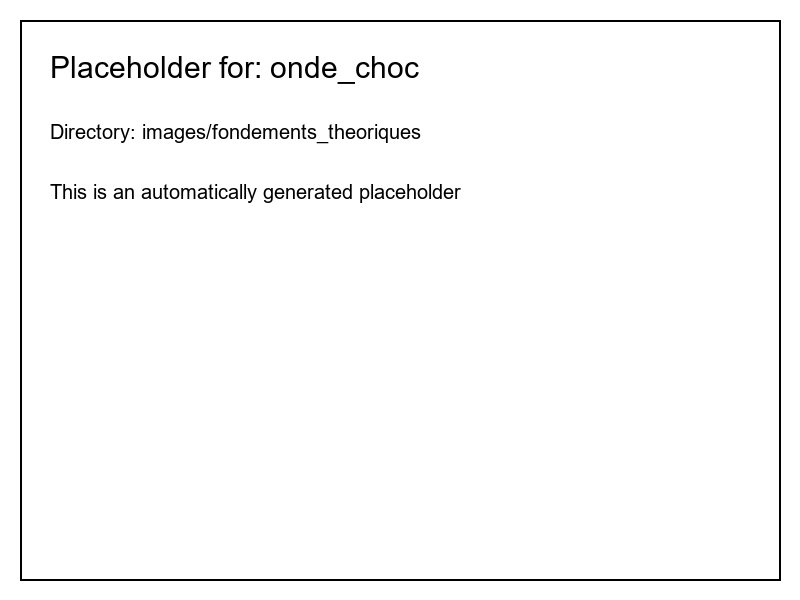
\includegraphics[width=0.8\textwidth]{images/fondements_theoriques/onde_choc}
\caption{Propagation d'une onde de choc : (a) représentation dans le plan $(x,t)$; (b) représentation sur le diagramme fondamental.}
\label{fig:onde_choc}
\end{figure}

\subsection{Problème de Riemann}
\label{subsec:riemann}

Le **problème de Riemann**, fondamental pour la résolution numérique de l'équation de conservation, consiste à déterminer l'évolution temporelle d'une discontinuité initiale. Il permet d'analyser comment des conditions initiales discontinues se résolvent en ondes de choc ou de raréfaction, fournissant ainsi une base pour comprendre des phénomènes de trafic complexes.

\begin{definition}[Problème de Riemann]
Le problème de Riemann pour l'équation de conservation du trafic consiste à résoudre :
\begin{align}
\pd{\dens}{t} + \pd{\flow(\dens)}{x} &= 0\\
\dens(x,0) &= 
\begin{cases}
\dens_L, & x < 0\\
\dens_R, & x > 0
\end{cases}
\end{align}
où $\dens_L$ et $\dens_R$ sont des constantes représentant les densités à gauche et à droite de la discontinuité initiale, respectivement.
\end{definition}

La solution du problème de Riemann dépend de la position relative des états $\dens_L$ et $\dens_R$ par rapport à la densité critique $\dens_c$ :

\begin{enumerate}
    \item Si $\dens_L < \dens_R < \dens_c$ ou $\dens_c < \dens_L < \dens_R$ : formation d'une **onde de choc**. Une onde de choc se forme lorsqu'une densité plus élevée rattrape une densité plus faible, créant une transition abrupte.
    \item Si $\dens_R < \dens_L < \dens_c$ ou $\dens_c < \dens_R < \dens_L$ : formation d'une **onde de raréfaction**. Une onde de raréfaction se forme lorsqu'une densité plus faible suit une densité plus élevée, créant une transition progressive.
    \item Si $\dens_L < \dens_c < \dens_R$ : formation d'une **onde de choc de congestion** (apparition d'un embouteillage). Dans ce cas, la densité à droite est suffisamment élevée pour provoquer une congestion qui se propage vers l'amont.
    \item Si $\dens_R < \dens_c < \dens_L$ : formation d'une **onde de raréfaction** (dissipation d'un embouteillage). Ici, la différence de densité favorise la dissipation de la congestion.
\end{enumerate}

Le modèle de Lighthill-Whitham-Richards (LWR) prédit que les véhicules passant à travers une zone de concentration accrue devront réduire leur vitesse de manière abrupte à l'entrée, créant une onde de choc. En revanche, ils pourront augmenter leur vitesse progressivement en sortant de cette zone.

Il convient de noter que d'autres modèles dits du second ordre peuvent tenir compte de l'accélération des conducteurs, offrant ainsi une représentation plus réaliste des transitions de vitesse, mais au prix d'une complexité mathématique accrue.

En pratique, les conditions initiales sont rarement aussi simples que celles du problème de Riemann, mais la compréhension de ses solutions est essentielle pour la conception d'algorithmes numériques robustes et précis.

\section{Limites du Modèle LWR Standard}
\label{sec:limites_lwr}

Malgré sa simplicité et son efficacité pour décrire les phénomènes macroscopiques du trafic, le modèle LWR standard présente plusieurs limitations qui rendent nécessaire son extension, particulièrement dans le contexte béninois :

\subsection{Homogénéité des Véhicules}
\label{subsec:homogeneite}

Le modèle LWR suppose que tous les véhicules sont identiques, ce qui ne reflète pas la réalité du trafic routier, et particulièrement pas celle du Bénin où cohabitent voitures, motos, camions, et autres types de véhicules.

\begin{remark}
Au Bénin, les motos représentent plus de 70\% du parc automobile, créant une dynamique de trafic très différente de celle modélisée par le LWR standard.
\end{remark}

\subsection{Relation Vitesse-Densité Unique}
\label{subsec:relation_unique}

Le modèle utilise une relation vitesse-densité unique pour tous les véhicules, ne tenant pas compte des différences de comportement entre classes de véhicules, ni de l'impact du type de revêtement routier sur la vitesse.

\subsection{Absence d'Interactions Complexes}
\label{subsec:interactions}

Le LWR ne modélise pas les interactions complexes entre différentes classes de véhicules, comme le comportement gap-filling des motos qui peuvent s'infiltrer entre les voitures.

\subsection{Modélisation Limitée des Intersections}
\label{subsec:intersections}

Le traitement des intersections et points singuliers du réseau n'est pas intégré de manière satisfaisante dans le modèle standard, alors qu'ils constituent des points critiques de la circulation urbaine au Bénin.

\section{Extensions Existantes du Modèle LWR}
\label{sec:extensions_existantes}

Différentes extensions du modèle LWR ont été proposées dans la littérature pour répondre à certaines de ses limitations :

\subsection{Modèles Multiclasses}
\label{subsec:multiclasses}

Les modèles multiclasses, comme ceux proposés par Wong et Wong \cite{wong2002multi}, étendent le LWR pour tenir compte de différentes classes de véhicules avec leurs propres caractéristiques (vitesse maximale, taille).

\begin{example}[Modèle de Wong et Wong]
Ce modèle propose un système d'équations couplées :
\begin{align}
\pd{\densi{i}}{t} + \pd{\flowi{i}}{x} &= 0, \quad \forall i \in \{1,\ldots,N\}\\
\veli{i} &= \veli{i}\left(\sum_{j=1}^{N} \densi{j}\right)
\end{align}
où les fonctions $\veli{i}$ tiennent compte de la densité totale.
\end{example}

\subsection{Modèles à Effets Non-locaux}
\label{subsec:non_local}

Ces modèles, comme celui de Zhang \cite{zhang2003non}, prennent en compte l'anticipation des conducteurs en intégrant une dépendance non-locale de la vitesse.

\subsection{Modèles de Transmission Cellulaire}
\label{subsec:cell_transmission}

Le modèle de transmission cellulaire de Daganzo \cite{daganzo1995cell} est une discrétisation du LWR qui facilite la modélisation des intersections et des réseaux complexes.

\section{Illustration Numérique du Modèle LWR}
\label{sec:illustration_numerique}

Pour compléter notre étude théorique et visualiser concrètement les phénomènes décrits précédemment (ondes de choc, raréfactions), nous avons implémenté une résolution numérique du modèle LWR. Les simulations présentées ci-dessous utilisent le schéma de Godunov, choisi pour sa capacité à préserver la nature conservative de l'équation et sa robustesse face aux discontinuités inhérentes aux problèmes de trafic. Contrairement à d'autres méthodes numériques, ce schéma évite l'apparition d'oscillations non physiques au voisinage des chocs tout en maintenant une précision satisfaisante. Les fondements mathématiques et détails d'implémentation de cette méthode sont présentés dans l'Annexe \ref{annexe:schemas_numeriques}.

\subsection{Schéma Numérique de Godunov}
\label{subsec:godunov}

Pour résoudre numériquement l'équation de conservation \eqref{eq:conservation_lwr}, nous discrétisons le domaine spatial en cellules de longueur $\Delta x$ et le temps en pas $\Delta t$. Le schéma de Godunov \cite{godunov1959finite,leveque1992numerical} se présente alors sous la forme :

\begin{equation}
\rho_i^{n+1} = \rho_i^n - \frac{\Delta t}{\Delta x}(F_{i+\frac{1}{2}} - F_{i-\frac{1}{2}})
\end{equation}

où $\rho_i^n$ représente la densité moyenne dans la cellule $i$ au temps $n\Delta t$, et $F_{i\pm\frac{1}{2}} sont les flux numériques aux interfaces entre les cellules. Ces flux sont déterminés en résolvant localement un problème de Riemann :

\begin{equation}
    F_{i+\frac{1}{2}} = \mathcal{F}(\rho_i^n, \rho_{i+1}^n)
\end{equation}
    
où $\mathcal{F}$ est la fonction de flux numérique de Godunov. Nous avons choisi ce schéma numérique car il est particulièrement adapté aux lois de conservation hyperboliques et permet de capturer précisément les discontinuités (ondes de choc) sans introduire d'oscillations parasites \cite{toro2013riemann}. Les détails complets concernant l'implémentation du schéma, les calculs des flux numériques et les preuves de convergence sont présentés dans l'Annexe \ref{annex:schemas_numeriques}.
    
\subsection{Scénarios de Simulation}
\label{subsec:scenarios}

Nous présentons ici trois scénarios caractéristiques qui illustrent les phénomènes fondamentaux du trafic routier modélisés par le LWR :

\begin{enumerate}
    \item \textbf{Feu rouge} : formation d'une congestion en amont d'un feu rouge et sa dissipation après le passage au vert.
    \item \textbf{Onde de choc} : rencontre d'un trafic rapide et d'un trafic lent créant une onde de choc se propageant en amont.
    \item \textbf{Onde de raréfaction} : accélération progressive d'un trafic initialement congestionné.
\end{enumerate}

\subsubsection{Feu Rouge}
\label{subsubsec:feu_rouge}

Considérons une route de 10 km où le trafic circule initialement à densité modérée ($\rho = 0,2\rho_{\max}$), mais avec un arrêt complet (densité proche de $\rho_{\max}$) au niveau d'un feu rouge situé à 5 km du début de la route. La Figure \ref{fig:feu_rouge} illustre l'évolution spatio-temporelle de la densité, de la vitesse et du flux après le passage du feu au vert.

\begin{figure}[htbp]
\centering
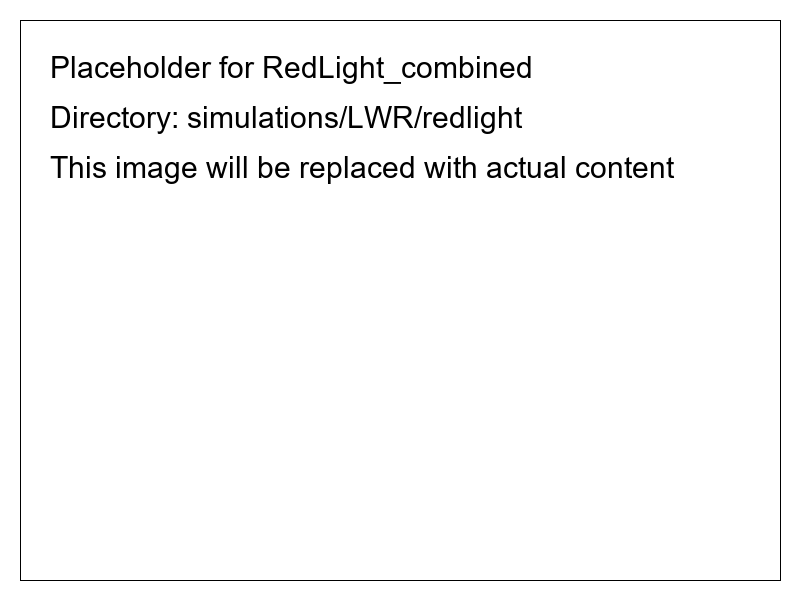
\includegraphics[width=1.0\textwidth]{simulations/LWR/redlight/RedLight_combined}
\caption{Simulation de la dissipation d'un embouteillage après le passage d'un feu au vert. De haut en bas : (a) Évolution de la densité, (b) Évolution de la vitesse, (c) Évolution du flux.}
\label{fig:feu_rouge}
\end{figure}

On observe clairement la formation d'une onde de choc qui se propage en amont du feu lorsque celui-ci est rouge, puis une onde de raréfaction qui se développe après le passage au vert. La vitesse de propagation de l'onde de choc correspond à la pente de la tangente au diagramme fondamental entre les états de trafic de part et d'autre du choc, comme prédit par la théorie.

\subsubsection{Onde de Choc}
\label{subsubsec:onde_choc_sim}

Dans ce scénario, nous simulons une route de 20 km avec un trafic fluide ($\rho = 0,1\rho_{\max}$) en amont et un trafic dense ($\rho = 0,7\rho_{\max}$) en aval. La Figure \ref{fig:sim_onde_choc} montre la formation et la propagation d'une onde de choc à l'interface entre ces deux régimes.

\begin{figure}[htbp]
\centering
\includegraphics[width=1.0\textwidth]{simulations/LWR/shock/ShockWave_combined}
\caption{Simulation de la formation et propagation d'une onde de choc. De haut en bas : (a) Évolution de la densité, (b) Évolution de la vitesse, (c) Évolution du flux.}
\label{fig:sim_onde_choc}
\end{figure}

On observe que l'onde de choc se propage en amont avec une vitesse négative constante, conformément à la théorie. Les véhicules doivent ralentir brusquement en atteignant le front de l'onde, ce qui correspond à une discontinuité dans le profil de vitesse.

\subsubsection{Onde de Raréfaction}
\label{subsubsec:rarefaction_sim}

Ce scénario illustre la dissipation progressive d'un embouteillage, représentée par une onde de raréfaction. Nous considérons une route de 20 km avec un trafic dense ($\rho = 0,7\rho_{\max}$) en amont et un trafic fluide ($\rho = 0,1\rho_{\max}$) en aval. La Figure \ref{fig:sim_rarefaction} montre l'évolution de cette situation.

\begin{figure}[htbp]
\centering
\includegraphics[width=1.0\textwidth]{simulations/LWR/rarefaction/RarefactionWave_combined}
\caption{Simulation d'une onde de raréfaction. De haut en bas : (a) Évolution de la densité, (b) Évolution de la vitesse, (c) Évolution du flux.}
\label{fig:sim_rarefaction}
\end{figure}

Contrairement à l'onde de choc, la transition est progressive : les véhicules accélèrent graduellement en sortant de la zone congestionnée, créant un éventail de caractéristiques dans le plan espace-temps.

\subsection{Limitations Révélées par les Simulations}
\label{subsec:limitations_sim}

Ces simulations, bien qu'illustrant correctement certains phénomènes de trafic, mettent en évidence plusieurs limitations du modèle LWR standard face aux spécificités du contexte béninois :

\begin{itemize}
    \item \textbf{Homogénéité des véhicules} : Les simulations supposent un flux homogène de véhicules identiques, ce qui ne reflète pas la diversité du parc automobile béninois dominé par les motos (zémidjans). La Figure \ref{fig:comparaison_flux} montre la différence entre un flux simulé homogène et des observations réelles à Cotonou, où la présence de motos crée des comportements de trafic distincts.
    
    \item \textbf{Comportement aux intersections} : Le modèle LWR standard ne peut pas simuler correctement les comportements spécifiques aux intersections non régulées fréquentes dans les villes béninoises, où les motos s'infiltrent entre les voitures et ne respectent pas nécessairement les files d'attente traditionnelles.
    
    \item \textbf{Effets de l'état des routes} : Les simulations ne tiennent pas compte de l'état variable des infrastructures routières, un facteur crucial au Bénin où la qualité du revêtement influe significativement sur les vitesses pratiquées.
\end{itemize}

Ces limitations, mises en évidence par la confrontation des simulations avec les observations de terrain, justifient pleinement la nécessité de développer une extension du modèle LWR adaptée aux spécificités du trafic routier béninois. Les fondements mathématiques rigoureux et les démonstrations formelles qui sous-tendent cette extension sont détaillés dans l'Annexe \ref{annexe:demonstrations}.

\begin{figure}[htbp]
\centering
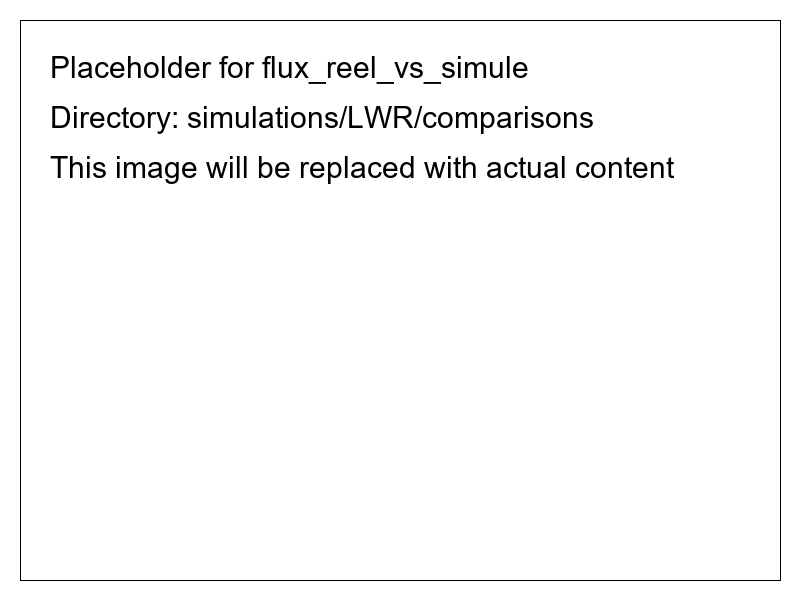
\includegraphics[width=0.8\textwidth]{simulations/LWR/comparisons/flux_reel_vs_simule}
\caption{Comparaison entre le flux simulé par le modèle LWR standard et des observations réelles dans une rue typique de Cotonou. Les différences significatives soulignent la nécessité d'adapter le modèle au contexte béninois.}
\label{fig:comparaison_flux}
\end{figure}

\section{Vers une Extension Adaptée au Contexte Béninois}
\label{sec:vers_extension}

L'extension que nous proposons vise à adapter le modèle LWR au contexte béninois en combinant et enrichissant plusieurs approches existantes :

\begin{itemize}
\item Adoption d'un cadre multiclasses pour distinguer les différents types de véhicules;
\item Introduction d'un coefficient de ralentissement lié au type de revêtement;
\item Développement de fonctions de modulation spécifiques pour les motos;
\item Traitement particulier des intersections et points singuliers.
\end{itemize}

Ces adaptations seront détaillées dans le Chapitre \ref{chap:extension_modele}, après une analyse approfondie des spécificités du réseau routier béninois et du rôle des motos dans le Chapitre \ref{chap:specificites_benin}.
